\documentclass[11pt]{article}
\usepackage{amsmath}
\usepackage{amssymb}
\usepackage{graphicx}
\usepackage{tabularx}
\usepackage{fancyhdr}
\usepackage{lastpage}

% Page layout
\usepackage[top=1in, bottom=1in, left=1in, right=1in]{geometry}

% Header and footer
\pagestyle{fancy}
\fancyhf{}
\rfoot{Page \thepage}
\renewcommand{\headrulewidth}{0pt}

% Modified Question command with left-aligned number
\newcommand{\questiona}[2]{
    \noindent\textbf{Q#2.} #1 \hfill \textbf{[1 Mark]}
}

\newcommand{\questionb}[2]{
    \noindent\textbf{Q#2.} #1 \hfill \textbf{[2 Marks]}
}

\begin{document}

% Title section with horizontal line
\begin{center}
    \Large\textbf{GATE 2018 - Agricultural Engineering (AG)} \\
    \large\textbf{General Aptitude and Technical Questions} \\
    \rule{\textwidth}{0.5pt} % Horizontal line below heading
\end{center}

\vspace{0.5cm}

% General Aptitude Section
\section*{General Aptitude}

\questiona{"When she fell down the \_\_\_\_\_, she received many \_\_\_\_\_ but little help." The words that best fill the blanks in the above sentence are}{1}
\begin{enumerate}
    \item[(A)] stairs, stares  
    \item[(B)] stairs, stairs  
    \item[(C)] stares, stairs  
    \item[(D)] stares, stares  
\end{enumerate}
\vspace{0.5cm}

\questiona{"In spite of being warned repeatedly, he failed to correct his \_\_\_\_\_ behaviour." The word that best fills the blank in the above sentence is}{2}
\begin{enumerate}
    \item[(A)] rational  
    \item[(B)] reasonable  
    \item[(C)] errant  
    \item[(D)] good  
\end{enumerate}
\vspace{0.5cm}

\questiona{For \(0 \leq x \leq 2\pi\), \(\sin x\) and \(\cos x\) are both decreasing functions in the interval \_\_\_\_\_.}{3}
\begin{enumerate}
    \item[(A)] \(\left(0, \frac{\pi}{2}\right)\)  
    \item[(B)] \(\left(\frac{\pi}{2}, \pi\right)\)  
    \item[(C)] \(\left(\pi, \frac{3\pi}{2}\right)\)  
    \item[(D)] \(\left(\frac{3\pi}{2}, 2\pi\right)\)  
\end{enumerate}
\vspace{0.5cm}

\questiona{The area of an equilateral triangle is \(\sqrt{3}\). What is the perimeter of the triangle?}{4}
\begin{enumerate}
    \item[(A)] 2  
    \item[(B)] 4  
    \item[(C)] 6  
    \item[(D)] 8  
\end{enumerate}
\vspace{0.5cm}

\questiona{Arrange the following three-dimensional objects in the descending order of their volumes:
\begin{enumerate}
    \item A cuboid with dimensions 10 cm, 8 cm and 6 cm
    \item A cube of side 8 cm
    \item A cylinder with base radius 7 cm and height 7 cm
    \item A sphere of radius 7 cm
\end{enumerate}}{5}
\begin{enumerate}
    \item[(A)] (i), (ii), (iii), (iv)  
    \item[(B)] (ii), (i), (iv), (iii)  
    \item[(C)] (iii), (ii), (i), (iv)  
    \item[(D)] (iv), (iii), (ii), (i)  
\end{enumerate}
\vspace{0.5cm}

\questionb{An automobile travels from city A to city B and returns to city A by the same route. The speed of the vehicle during the onward and return journeys were constant at 60 km/h and 90 km/h, respectively. What is the average speed in km/h for the entire journey?}{6}
\begin{enumerate}
    \item[(A)] 72  
    \item[(B)] 73  
    \item[(C)] 74  
    \item[(D)] 75  
\end{enumerate}
\vspace{0.5cm}

\questionb{A set of 4 parallel lines intersect with another set of 5 parallel lines. How many parallelograms are formed?}{7}
\begin{enumerate}
    \item[(A)] 20  
    \item[(B)] 48  
    \item[(C)] 60  
    \item[(D)] 72  
\end{enumerate}
\vspace{0.5cm}

\questionb{To pass a test, a candidate needs to answer at least 2 out of 3 questions correctly. A total of 6,30,000 candidates appeared for the test. Question A was correctly answered by 3,30,000 candidates. Question B was answered correctly by 2,50,000 candidates. Question C was answered correctly by 2,60,000 candidates. Both questions A and B were answered correctly by 1,00,000 candidates. Both questions B and C were answered correctly by 90,000 candidates. Both questions A and C were answered correctly by 80,000 candidates. If the number of students answering all questions correctly is the same as the number answering none, how many candidates failed to clear the test?}{8}
\begin{enumerate}
    \item[(A)] 30,000  
    \item[(B)] 2,70,000  
    \item[(C)] 3,90,000  
    \item[(D)] 4,20,000  
\end{enumerate}
\vspace{0.5cm}

\questionb{If \(x^2 + x - 1 = 0\) what is the value of \(x^4 + \frac{1}{x^4}\)?}{9}
\begin{enumerate}
    \item[(A)] 1  
    \item[(B)] 5  
    \item[(C)] 7  
    \item[(D)] 9  
\end{enumerate}
\vspace{0.5cm}

\questionb{In a detailed study of annual crow births in India, it was found that there was relatively no growth during the period 2002 to 2004 and a sudden spike from 2004 to 2005. In another unrelated study, it was found that the revenue from cracker sales in India which remained fairly flat from 2002 to 2004, saw a sudden spike in 2005 before declining again in 2006. The solid line in the graph below refers to annual sale of crackers and the dashed line refers to the annual crow births in India. Choose the most appropriate inference from the above data.}{10}

\begin{center}
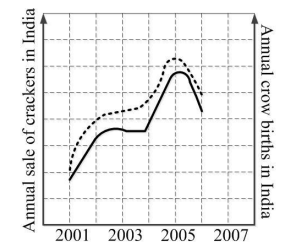
\includegraphics[width=0.5\textwidth]{figures/10.png}
\end{center}

\begin{enumerate}
    \item[(A)] There is a strong correlation between crow birth and cracker sales.
    \item[(B)] Cracker usage increases crow birth rate.
    \item[(C)] If cracker sale declines, crow birth will decline.
    \item[(D)] Increased birth rate of crows will cause an increase in the sale of crackers.
\end{enumerate}
\vspace{0.5cm}

% Technical Section
\section*{Technical Section}

\questiona{The general solution to the second order linear homogeneous differential equation \( y'' - 6y' + 25y = 0 \) is}{1}
\begin{enumerate}
    \item[(A)] \( e^{3x} \) (a \(\cos 4x + b \sin 4x\))  
    \item[(B)] \( e^{31x} \) (a \(\cos 4x + b \sin 4x\))  
    \item[(C)] \( e^{4x} \) (a \(\cos 3x + b \sin 3x\))  
    \item[(D)] \( e^{41x} \) (a \(\cos 3x + b \sin 3x\))  
\end{enumerate}
\vspace{0.5cm}

\questiona{Solution of \( f(x) = x^4 + 2x^3 - 4x^2 + 3x - 1 = 0 \) is}{2}
\begin{enumerate}
    \item[(A)] 0.333  
    \item[(B)] 0.646  
    \item[(C)] 0.658  
    \item[(D)] 1.000  
\end{enumerate}
\vspace{0.5cm}

\questiona{Integration of \[ \int_0^D \frac{D}{2} \frac{2R^2 x \, dx}{(R^2 + x^2)^2} \] is}{3}
\begin{enumerate}
    \item[(A)] \[ \frac{R^2}{R^2 + D^2} \]  
    \item[(B)] \[ \frac{4R^2}{4R^2 + D^2} \]  
    \item[(C)] \[ \frac{D^2}{R^2 + D^2} \]  
    \item[(D)] \[ \frac{D^2}{4R^2 + D^2} \]  
\end{enumerate}
\vspace{0.5cm}

\questiona{The type of the sequence \( a_n = \left( \frac{n}{n-1} \right)^3 \) is}{4}
\begin{enumerate}
    \item[(A)] oscillatory  
    \item[(B)] bounded  
    \item[(C)] converging  
    \item[(D)] diverging  
\end{enumerate}
\vspace{0.5cm}

\questiona{For accepting or rejecting a null hypothesis, which one of the following is NOT used as a significance test method in statistics?}{5}
\begin{enumerate}
    \item[(A)] Z-test  
    \item[(B)] Student's t-test  
    \item[(C)] Pearson's correlation  
    \item[(D)] Relative standard deviation  
\end{enumerate}
\vspace{0.5cm}

\questiona{For a two-wheel drive tractor, use of differential lock in adverse field condition ensures}{6}
\begin{enumerate}
    \item[(A)] equal distribution of torque to both the drive wheels.  
    \item[(B)] equal distribution of power to both the drive wheels.  
    \item[(C)] distribution of higher amount of torque to the wheel under poor traction.  
    \item[(D)] distribution of higher amount of torque to the wheel under better traction.  
\end{enumerate}
\vspace{0.5cm}

\questiona{During field evaluation of a combine harvester, total grain collected at the grain tank was 135 kg. Amount of threshed grain found over walker and shoe were 0.65 kg and 2.4 kg, respectively. Unthreshed grain lost with straw and chaff were 4.54 kg and 0.28 kg, respectively. Threshing efficiency of the combine harvester in percent is}{7}
\begin{enumerate}
    \item[(A)] 94.37  
    \item[(B)] 94.49  
    \item[(C)] 96.50  
    \item[(D)] 96.63  
\end{enumerate}
\vspace{0.5cm}

\questiona{Match the following items of Column I with the corresponding items of Column II:}{8}
\begin{center}
\begin{tabular}{|l|l|l|l|}
\hline
 & Column I & & Column II \\
\hline
P. & Cetane number & 1. & Beam radiation \\
Q. & Pyrheliometer & 2. & Anti-knock quality \\
R. & Octane number & 3. & Total solar radiation \\
S. & Pyranometer & 4. & Ignition quality \\
\hline
\end{tabular}
\end{center}
\begin{enumerate}
    \item[(A)] P-2, Q-3, R-1, S-4  
    \item[(B)] P-4, Q-1, R-2, S-3  
    \item[(C)] P-4, Q-3, R-2, S-1  
    \item[(D)] P-2, Q-4, R-1, S-3  
\end{enumerate}
\vspace{0.5cm}

\questiona{Constituents of the producer gas contributing to its heating value are}{9}
\begin{enumerate}
    \item[(A)] CO and $CO_2$ 
    \item[(B)] $CH_4$ and $CO_2$  
    \item[(C)] CO and $H_2$  
    \item[(D)] $CO_2$ and $H_2$  
\end{enumerate}
\vspace{0.5cm}

\questiona{One of the key assumptions made by Dupuit-Forchheimer about the flow behavior in the porous medium towards subsurface drains is}{10}
\begin{enumerate}
    \item[(A)] homogeneous medium  
    \item[(B)] isotropic medium  
    \item[(C)] horizontal streamlines  
    \item[(D)] uniform recharge  
\end{enumerate}
\vspace{0.5cm}

\questiona{The depths from the soil surface to subsurface tile drains, impermeable soil layer and the highest water table are measured as 2.8 m, 5.0 m and 0.8 m, respectively. The effective hydraulic head for drainage in meter is}{11}
\begin{enumerate}
    \item[(A)] 0.8  
    \item[(B)] 2.0  
    \item[(C)] 2.2  
    \item[(D)] 4.2  
\end{enumerate}
\vspace{0.5cm}

\questiona{The discharge from a sprinkler nozzle depends on}{12}
\begin{enumerate}
    \item[(A)] operating pressure and nozzle geometry.  
    \item[(B)] operating pressure and distribution pattern.  
    \item[(C)] application rate and nozzle angle.  
    \item[(D)] operating pressure and application rate.  
\end{enumerate}
\vspace{0.5cm}

\questiona{If the void ratio of a soil column is 0.43, the soil porosity is}{13}
\begin{enumerate}
    \item[(A)] 0.30  
    \item[(B)] 0.40  
    \item[(C)] 0.70  
    \item[(D)] 0.75  
\end{enumerate}
\vspace{0.5cm}

\questiona{Which one of the following is a WRONG statement?}{14}
\begin{enumerate}
    \item[(A)] The head generated by a centrifugal pump at zero discharge is the 'shutoff head'.  
    \item[(B)] To avoid cavitation in centrifugal pumps, the net positive suction head should be more than the theoretical atmospheric pressure.  
    \item[(C)] According to the affinity laws of centrifugal pumps, the head varies with the square of the impeller speed.  
    \item[(D)] Most of the turbine pumps have operational characteristics closer to those of the centrifugal pumps than the propeller pumps.  
\end{enumerate}
\vspace{0.5cm}

\questiona{If the departure and latitude of a line during Theodolite survey are 70.03 m and -100 m, respectively, the whole circle bearing of this line in degree is}{15}
\begin{enumerate}
    \item[(A)] 55  
    \item[(B)] 125  
    \item[(C)] 135  
    \item[(D)] 145  
\end{enumerate}
\vspace{0.5cm}

\questiona{Convective film heat transfer coefficient (h) of air (thermal conductivity=0.025 W m\(^{-1}\) K\(^{-1}\)) in W m\(^{-2}\) K\(^{-1}\), trapped between two parallel glass panes in a window 1.5 mm apart, is}{16}
\begin{enumerate}
    \item[(A)] 3.75  
    \item[(B)] 16.67  
    \item[(C)] 37.52  
    \item[(D)] 60.21  
\end{enumerate}
\vspace{0.5cm}

\questiona{Log mean temperature difference (LMTD) correction factor (F) is applicable to}{17}
\begin{enumerate}
    \item[(A)] Spiral tube heat exchanger  
    \item[(B)] Steam jacketed kettle  
    \item[(C)] Plate heat exchanger  
    \item[(D)] Evaporator tubes  
\end{enumerate}
\vspace{0.5cm}

\questiona{Which one of the following statements related to parboiling of paddy is NOT correct?}{18}
\begin{enumerate}
    \item[(A)] Irreversible granule swelling occurs during heating.  
    \item[(B)] Parboiling process is used to salvage wet or damaged paddy.  
    \item[(C)] Parboiled rice takes less time to cook as compared to raw rice due to starch gelatinization.  
    \item[(D)] Milling yield of paddy increases due to starch gelatinization.  
\end{enumerate}
\vspace{0.5cm}

\questiona{In refining of the rice bran oil for edible purpose, neutralization process is carried out mainly to remove}{19}
\begin{enumerate}
    \item[(A)] wax and organic impurities  
    \item[(B)] gums and mucilage  
    \item[(C)] saturated glycerides  
    \item[(D)] free fatty acids  
\end{enumerate}
\vspace{0.5cm}

\questiona{Which one of the following chemicals is NOT used for fumigation in either horizontal or vertical storage structures to kill insects?}{20}
\begin{enumerate}
    \item[(A)] Methyl bromide  
    \item[(B)] Phosphine  
    \item[(C)] Phostoxin  
    \item[(D)] Silver sulphate  
\end{enumerate}
\vspace{0.5cm}

\questiona{Match the following agricultural/food by-products in Column I with their respective value added products in Column II.}{21}
\begin{center}
\begin{tabular}{|l|l|l|l|}
\hline
 & Column I & & Column II \\
\hline
P. & Banana pseudostem & 1. & Silicon tetrachloride \\
Q. & Coconut shell & 2. & Protein food \\
R. & Meat waste & 3. & Starch \\
S. & Rice husk & 4. & Furfural \\
\hline
\end{tabular}
\end{center}
\begin{enumerate}
    \item[(A)] P-2, Q-3, R-1, S-4  
    \item[(B)] P-3, Q-4, R-2, S-1  
    \item[(C)] P-4, Q-3, R-2, S-1  
    \item[(D)] P-3, Q-1, R-2, S-4  
\end{enumerate}
\vspace{0.5cm}

\questiona{An epicyclic gear train consists of a sun gear, four planet gears pinned on a planet carrier (which is mounted on the sun gear) and a fixed ring gear (in which the entire sun-planet gear assembly is inserted). If the ring gear has 56 teeth and each planet gear has 18 teeth, the number of teeth on the sun gear is \_\_\_\_\_.}{22}
\vspace{0.5cm}

\questiona{A self-propelled power reaper with a 1.2 m wide cutter bar was operated at a forward speed of 4 km h\(^{-1}\). Turning loss during operation was observed to be 25 minutes per hectare. Neglecting any other losses, the field efficiency of the reaper will be \_\_\_\_\_\%.}{23}
\vspace{0.5cm}

\questiona{The porosity and compressibility of a 7.8 m thick confined aquifer are 0.25 and 1×10\(^{-8}\) m\(^{2}\) N\(^{-1}\), respectively. The storage coefficient of the aquifer is 6.5×10\(^{-4}\). To release 650 m\(^{3}\) of water from 1 km\(^{2}\) of this aquifer, the average decline in hydraulic head will be \_\_\_\_\_ m.}{24}
\vspace{0.5cm}

\questiona{Molecular diffusivity (D\(_{AB}\)) of water vapour in air is 2.6×10\(^{-5}\) m\(^{2}\) s\(^{-1}\) over an effective distance of 3 mm. Density and coefficient of viscosity of air are 1.2 kg m\(^{-3}\) and 2×10\(^{-5}\) kg m\(^{-1}\) s\(^{-1}\), respectively. Sherwood Number (N\(_{sh}\)) for water vapour in air is \_\_\_\_\_.}{25}
\vspace{0.5cm}

\questionb{Rank of a matrix 
\[
\begin{bmatrix}
5 & 3 & -3 & -1 \\
3 & 2 & -2 & -1 \\
2 & -1 & 2 & 8
\end{bmatrix}
\] is}{26}
\begin{enumerate}
    \item[(A)] 1  
    \item[(B)] 2  
    \item[(C)] 3  
    \item[(D)] 4  
\end{enumerate}
\vspace{0.5cm}

\questionb{A particle is subjected to forces \( P = 2i - 5j + 6k \) and \( Q = -i + 2j - k \). The positional vectors are \( \vec{OA} = 4i - 3j - 2k \) and \( \vec{OB} = 6i + j - 3k \). Work done by the resultant force (\( F = P + Q \)) to move the particle from A to B is}{27}
\begin{center}
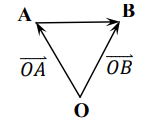
\includegraphics[width=0.5\textwidth]{figures/27.png}
\end{center}

\begin{enumerate}
    \item[(A)] 2  
    \item[(B)] -5  
    \item[(C)] 12  
    \item[(D)] -15  
\end{enumerate}
\vspace{0.5cm}

\questionb{A two-wheel drive tractor weighing 18 kN has a wheel base 1.8 m. Its centre of gravity is located 600 mm ahead of the rear axle centre, under static condition, on a level ground. When this tractor is used to pull a disc plough hitched at a height of 390 mm from the ground, the draft observed is 6 kN. The change in reaction on rear wheels of the tractor due to pull in kN is}{28}
\begin{enumerate}
    \item[(A)] 1.30  
    \item[(B)] 1.95  
    \item[(C)] 3.90  
    \item[(D)] 5.85  
\end{enumerate}
\vspace{0.5cm}

\questionb{Match the following items in Column I with the corresponding items in Column II:}{29}
\begin{center}
\begin{tabular}{|l|l|l|l|}
\hline
 & Column I & & Column II \\
\hline
P. & Flownet & 1. & Soil erosion \\
Q. & Elso Index & 2. & Curve number \\
R. & Groynes & 3. & Equipotential line \\
S. & Isobath & 4. & Groundwater \\
T. & Runoff & 5. & River bank \\
\hline
\end{tabular}
\end{center}
\begin{enumerate}
    \item[(A)] P-4, Q-2, R-5, S-3, T-1  
    \item[(B)] P-4, Q-3, R-1, S-5, T-2  
    \item[(C)] P-3, Q-1, R-5, S-4, T-2  
    \item[(D)] P-3, Q-1, R-2, S-4, T-5  
\end{enumerate}
\vspace{0.5cm}

\questionb{The velocity (v) of a tractor, which starts from rest, is given at fixed intervals of time (t) as follows:}{30}
\begin{center}
\begin{tabular}{|c|c|c|c|c|c|c|c|c|c|c|c|}
\hline
t (min) & 0 & 2 & 4 & 6 & 8 & 10 & 12 & 14 & 16 & 18 & 20 \\
\hline
v (m min\(^{-1}\)) & 0 & 0.8 & 1.5 & 2.1 & 2.4 & 2.7 & 1.7 & 0.9 & 0.4 & 0.2 & 0 \\
\hline
\end{tabular}
\end{center}
Using Simpson's \(1/3^{rd}\) rule, the distance covered by the tractor in 20 minutes will be \_\_\_\_\_ m.
\vspace{0.5cm}

\questionb{In a box, there are 2 red, 3 black and 4 blue coloured balls. The probability of drawing 2 blue balls in sequence without replacing, and then drawing 1 black ball from this box is \_\_\_\_\_ \%.}{31}
\vspace{0.5cm}

\questionb{An open belt drive system transmits 5 kW power using a flat belt of width and thickness as 80 mm and 5 mm, respectively. The driving shaft speed is 1500 rpm and the driven shaft speed is 500 rpm. The coefficient of friction between the belt and pulley is 0.20, and the wrap angle of the belt is 168°. If diameter of the smaller pulley is 200 mm, maximum stress induced in the belt will be \_\_\_\_\_ MPa.}{32}
\vspace{0.5cm}

\questionb{A 2 m\(^3\) biogas plant is to be operated using cow-dung as feedstock. The cow-dung is mixed with water in proportion of 1:1 (by weight) to form a slurry of density 1090 kg m\(^{-3}\). The yield of biogas is 0.036 m\(^3\) kg\(^{-1}\) of cow-dung. If the hydraulic retention time is 40 days, volume of the digester of the biogas plant will be \_\_\_\_\_ m\(^3\).}{33}
\vspace{0.5cm}

\questionb{A power tiller with diesel engine produces 12 kW of brake power with a brake thermal efficiency of 30\%. If the air-fuel ratio in the combustion process is 14:1 and heating value of the fuel is 45 MJ kg\(^{-1}\), air consumption rate of the engine will be \_\_\_\_\_ kg h\(^{-1}\).}{34}
\vspace{0.5cm}

\questionb{Air enters into an engine cylinder at a pressure of 100 kPa and temperature of 300 K in the suction stroke of an ideal Otto cycle. The cylinder clearance volume is 600 cm\(^3\) and compression ratio is 8:1. The expansion stroke of the cycle is polytropic in nature. The pressure at the beginning of the expansion stroke is 10 MPa and the temperature at the end of the expansion stroke is 1800 K. The polytropic exponent of the expansion stroke is \_\_\_\_\_.}{35}
\vspace{0.5cm}

\questionb{A tractor drawn five-time sweep type cultivator is set at an angle (load angle) of 45° with the soil surface during its operation. The sweep of each fine experiences a normal force of 960 N on its surface. If the coefficient of soil-metal friction is 0.3, the total draft requirement of the cultivator is \_\_\_\_\_ kN.}{36}
\vspace{0.5cm}

\questionb{A two-wheel drive tractor with rear wheel rolling radius of 600 mm develops a tractive force of 18.5 kN at a wheel slip of 12\%. The engine speed is 2400 rpm and the transmission ratio from the engine to the rear wheels is 120:1. If the tractor experiences a motion resistance of 1.75 kN, the drawbar power developed by the tractor will be \_\_\_\_\_ kW.}{37}
\vspace{0.5cm}

\questionb{A single plate dry clutch transmits 15 kW power at 1200 rpm. The clutch sustains a maximum axial load of 2.65 kN. The ratio of outer to inner diameter of the frictional surface is 1.25:1. Considering uniform wear with a coefficient of friction of 0.3 on both the frictional surfaces, the outer diameter of the clutch plate is \_\_\_\_\_ mm.}{38}
\vspace{0.5cm}

\questionb{A precision seed planter can plant 10 seeds per revolution of the metering plate with a row to row distance of 450 mm at a speed of 6 km h\(^{-1}\). A plant population of 36 plants per square meter is desired for the crop. The germination percentage of the seed is 90\%. If the planter ground wheel has a rolling radius of 350 mm, the speed ratio of metering plate to the ground wheel required to obtain the desired plant population is \_\_\_\_\_.}{39}
\vspace{0.5cm}

\questionb{The elevations of pressure gauge and porous cup of the tensiometer installed in unsaturated zone are 145.8 m and 144.2 m, respectively. Pressure measured at the gauge is -19.62×10\(^3\) N m\(^{-2}\). The specific weight of water is 9810 N m\(^{-3}\). The estimated pressure at the porous cup is \_\_\_\_\_ N m\(^{-2}\).}{40}
\vspace{0.5cm}

\questionb{The drawdown at the well face of a 30 cm diameter fully penetrating well in a confined aquifer is 3 m. The radius of influence of this well is 3 km. For the same discharge and aquifer condition, the drawdown at 300 m away from the centre of the well is \_\_\_\_\_ m.}{41}
\vspace{0.5cm}

\questionb{A permanent matured orchard has a tree spacing of 4 m×5 m. Each tree has a shading area of 40\% to be irrigated with the 'pig tail' pattern multi-exit drip emitters. The effective wetting geometry of each emitter is 2 m×2 m. The emitters have discharge constant and exponent of 0.3 and 0.6, respectively. The coefficient of variation of emitter discharge is 0.06. The average and minimum operating pressures are 120 kPa and 100 kPa, respectively. The emission uniformity of the emitters is \_\_\_\_\_ \%.}{42}
\vspace{0.5cm}

\questionb{The 6-hour unit hydrograph of a watershed is represented by an isosceles triangle with the peak of 180 m\(^3\) s\(^{-1}\) and time to peak of 18 hours. The phi-index (\(\phi\)) of this watershed is 3.0 mm h\(^{-1}\) and the constant baseflow is 20 m\(^3\) s\(^{-1}\). The accumulated rainfall received in this watershed at 6 h and 12 h from the start of the storm are 38 mm and 106 mm, respectively. The resulting peak of the flood hydrograph due to this storm event is \_\_\_\_\_ m\(^3\) s\(^{-1}\).}{43}
\vspace{0.5cm}

\questionb{Three geometrically identical Lysimeters (A, B and C) installed in a paddy field have uniform initial ponding depths of 12 cm. After a week, the recorded water depths in A, B and C are 10.4 cm, 8.6 cm, and 7.0 cm, respectively. Rainfall received during this week is 15 mm, and the crop coefficient of paddy is 0.94. Lysimeter 'A' has a closed bottom with no plant. Lysimeter 'B' has an open bottom with no plant. Lysimeter 'C' has an open bottom with paddy plants. Neglecting the boundary effects and groundwater contribution in the Lysimeters, the weekly potential evapotranspiration will be \_\_\_\_\_ cm.}{44}
\vspace{0.5cm}

\questionb{A rectangular chute spillway is designed for gully erosion control with a drop (H) of 5 m, peak flow of 1.81 m\(^3\) s\(^{-1}\) and maximum inlet water level of 0.81 m. Frictional head loss over the apron is 20\% of H. The design height of chute blocks is equal to the depth of flow in the water way. Acceleration due to gravity (g) is 9.81 m s\(^{-2}\). If coefficient of discharge of the weir section is 1.66, height of the chute blocks is \_\_\_\_\_ m.}{45}
\vspace{0.5cm}

\questionb{Furrows of 120 m length with 0.5\% slope are made at 90 cm spacing. The maximum non-erosive stream flow rate is applied in a furrow that takes 1.0 hour to reach the lower end. Then this flow rate is reduced to half of its size and, subsequently, continued for another 1.0 hour. The average depth of applied water is \_\_\_\_\_ cm.}{46}
\vspace{0.5cm}

\questionb{A cylindrical tank of 1.5 m diameter and 4 m height is filled with a liquid by a pipe of 2.5 cm internal diameter. The density and dynamic viscosity of the liquid are 1050 kg m\(^{-3}\) and 1.6×10\(^{-3}\) N s m\(^{-2}\), respectively. If flow in the pipe is turbulent, the maximum time required to fill the tank is \_\_\_\_\_ hours.}{47}
\vspace{0.5cm}

\questionb{In a falling film evaporator, the inside and outside diameters of the tube wall are 25 mm and 27 mm, respectively. The tube is made of SS304 (thermal conductivity=15 W m\(^{-1}\) K\(^{-1}\)) and the inside convective film coefficient is 750 W m\(^{-2}\) K\(^{-1}\). Outside the tube wall, film coefficient of condensing steam is 7175 W m\(^{-2}\) K\(^{-1}\). Based on the inside area of the tube, the overall heat transfer coefficient is \_\_\_\_\_ W m\(^{-2}\) K\(^{-1}\).}{48}
\vspace{0.5cm}

\questionb{Mass flow rate of outside air through a duct is 735 kg h\(^{-1}\). Absolute humidity of air is 0.025 kg water vapour per kg dry air at 40°C. This air is mixed with equal quantity of moist exhaust air coming out of a counter current dryer at 55°C. The mixed air is heated up to 75°C to dry barley, fed at 174 kg h\(^{-1}\), at an initial moisture content of 31\% (wet basis) to a final value of 7\% (dry basis). The absolute humidity of the exhaust air from the dryer in 'kg water vapour per kg dry air' will be \_\_\_\_\_.}{49}
\vspace{0.5cm}

\questionb{One ton of marine fishery products are to be brought down from 32°C temperature to -18°C in half an hour time using a plate freezer. The freezing point of 85\% water (based on total mass of the product) present in the fish is -0.3°C. Specific heat capacities of fresh and frozen fish solids (15\% of total mass) are 3.2 and 1.8 kJ kg\(^{-1}\) K\(^{-1}\), respectively. Specific heat capacity of fresh water is 4.2 kJ kg\(^{-1}\) K\(^{-1}\) and that of ice is 2.2 kJ kg\(^{-1}\) K\(^{-1}\). Latent heat of crystallization of water is 335 kJ kg\(^{-1}\). For freezing the products, the compressor power consumption with a vapour compression refrigeration cycle (coefficient of performance, 3.66) is \_\_\_\_\_ kW.}{50}
\vspace{0.5cm}

\questionb{Mycobacterium tuberculosis is having decimal reduction time of 13.5 s at 72°C. The count of the organism is to be reduced by eight logarithmic cycles in milk pasteurization with adequate holding at a temperature of 85°C. If Q\(_{10}\) value for the organism is 7.5, the minimum holding time for the desired sterility of this particular organism at 85°C is \_\_\_\_\_ seconds.}{51}
\vspace{0.5cm}

\questionb{A horizontal screw conveyor of length 3.2 m conveys solid grain having bulk density of 725 kg m\(^{-3}\). The screw diameter, shaft diameter and pitch of the screw are 0.6 m, 0.24 m and 0.48 m, respectively. If the screw is operating with 80\% of its volumetric capacity at a speed of 50 rpm, the actual discharge of the screw is \_\_\_\_\_ ton h\(^{-1}\).}{52}
\vspace{0.5cm}

\questionb{In a feed milling plant, it has been observed that 80\% of the feed passes through IS sieve 340 (3.25 mm opening) and 80\% of the ground feed passes through IS sieve 40 (0.42 mm opening). The power requirement to crush the material with a feed rate of 3 ton h\(^{-1}\) is 6 kW. Power requirement to crush 2 ton h\(^{-1}\) of the same feed using the above system so that 80\% of the ground feed pass through IS sieve 15 (opening 0.157 mm) is \_\_\_\_\_ kW.}{53}
\vspace{0.5cm}

\questionb{Solid food particles having nominal size of 0.2 mm with shape factor of 0.8 and density of 1040 kg m\(^{-3}\) are to be fluidized using air at 28°C. The density and pressure of air at the above-mentioned condition are 1.175 kg m\(^{-3}\) and 1.013×10\(^5\) Pa, respectively. The voidage at minimum fluidizing condition is 0.48. Use the value of 'g' as 9.81 m s\(^{-2}\). If cross section of the empty bed is 0.5 m\(^2\) and contains 520 kg of solids, the pressure drop at minimum fluidization condition is \_\_\_\_\_ kPa.}{54}
\vspace{0.5cm}

\questionb{A single strength fruit juice is concentrated from 6\% total solids (TS) to 24\% by ultrafiltration. The feed stream has a flow rate of 12 kg min\(^{-1}\). The ultrafiltration membrane tube has an inside diameter of 80 mm and the pressure difference applied across the membrane is 2 MPa. If the permeability constant is 4×10\(^{-5}\) kg water m\(^{-2}\) kPa\(^{-1}\) s\(^{-1}\), the length of the membrane tube is \_\_\_\_\_ m.}{55}
\vspace{0.5cm}

\begin{center}
\textbf{END OF THE QUESTION PAPER}
\rule{\textwidth}{0.5pt} 
\end{center}
\end{document}
